\documentclass[a4paper]{article}
\usepackage[utf8]{inputenc}
\usepackage[spanish, es-tabla, es-noshorthands]{babel}
\usepackage[table,xcdraw]{xcolor}
\usepackage[a4paper, footnotesep = 1cm, width=20cm, top=2.5cm, height=25cm, textwidth=18cm, textheight=25cm]{geometry}
%\geometry{showframe}

\usepackage{tikz}
\usepackage{amsmath}
\usepackage{amsfonts}
\usepackage{amssymb}
\usepackage{float}
\usepackage{graphicx}
\usepackage{caption}
\usepackage{subcaption}
\usepackage{multicol}
\usepackage{multirow}
\setlength{\doublerulesep}{\arrayrulewidth}
\usepackage{booktabs}

\usepackage{hyperref}
\hypersetup{
    colorlinks=true,
    linkcolor=blue,
    filecolor=magenta,      
    urlcolor=blue,
    citecolor=blue,    
}

\newcommand{\quotes}[1]{``#1''}
\usepackage{array}
\newcolumntype{C}[1]{>{\centering\let\newline\\\arraybackslash\hspace{0pt}}m{#1}}
\usepackage[american]{circuitikz}
\usetikzlibrary{calc}
\usepackage{fancyhdr}
\usepackage{units} 
\usepackage{svg}

\graphicspath{{../Ejercicio-1/}{../Ejercicio-2/}{../Ejercicio-3/}{../Ejercicio-4/}{../Ejercicio-5/}}
%\svgpath{{../Ejercicio-1/}{../Ejercicio-2/}{../Ejercicio-3/}{../Ejercicio-4/}{../Ejercicio-5/}}

\pagestyle{fancy}
\fancyhf{}
\lhead{22.05 ASSD}
\rhead{Mechoulam, Lambertucci, Rodriguez, Londero}
\rfoot{Página \thepage}

\begin{document}

\subsection{Introducción}
Se pidió investigar soluciones para la interconexión de un sistemas TTL de 5V con uno de 3.3V. Para esto proponemos dos soluciones.\\
La primera es la utilización de TTL\footnote{Transistor Transistor Logic} y LVTTL\footnote{Low Voltage Transistor Transistor Logic} tal que los voltages queden de la siguiente manera siendo compatibles entre sí.\\
\begin{figure}[H]
  \centering
  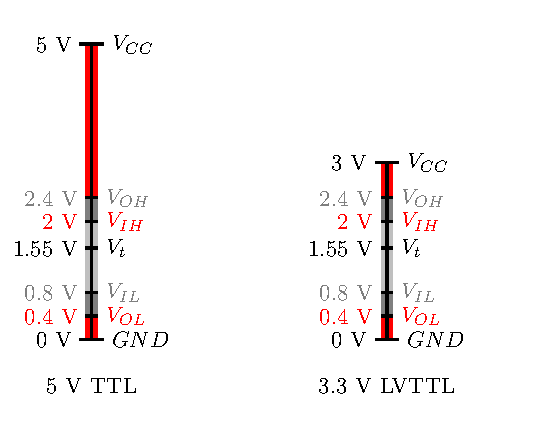
\includegraphics[width=.6\textwidth, page = 1]{ImagenesEjercicio4/Draw.pdf}
  \caption{Niveles Lógicos TTL y LVTTL}.
  \label{fig:ttlLvl}
\end{figure}
La segunda es la implementación de un Level Shifter mediante un transistor MOS y dos resistencias \ref{fig:LVSH}, esta configuraicón permite la traducción de los niveles lógicos en ambos sentidos.
\begin{figure}[H]
  \centering
  \includegraphics[width=.6\textwidth, page = 2]{ImagenesEjercicio4/Draw.pdf}
  \caption{Level Shifter}.
  \label{fig:LVSH}
\end{figure}

\end{document}